\documentclass[11pt]{article}

% ---- packages ----
\usepackage[margin=1in]{geometry}
\usepackage{amsmath,amssymb}
\usepackage{booktabs}
\usepackage{array}
\usepackage{xcolor}
\usepackage{tikz}
\usetikzlibrary{arrows.meta,positioning,shapes.geometric,fit,backgrounds}
\usepackage[hidelinks]{hyperref}
\usepackage{enumitem}
\usepackage{microtype}
\usepackage[htt]{hyphenat}   % allow long \texttt{} tokens to break across lines
\usepackage{seqsplit}        % break-anywhere for long identifiers in narrow table cells

% ---- styling ----
\definecolor{unityblue}{HTML}{2C5F9E}
\definecolor{pyorange}{HTML}{C9560B}
\definecolor{codegray}{HTML}{555555}
% \color switch (not \textcolor) so the \texttt argument is NOT boxed and can break/hyphenate
\newcommand{\code}[1]{{\texttt{\small #1}}}
\newcommand{\unity}[1]{{\color{unityblue}\texttt{\small #1}}}
\newcommand{\py}[1]{{\color{pyorange}\texttt{\small #1}}}
\newcommand{\clip}{\operatorname{clip}_{[0,1]}}

\title{\textbf{Reward Scoring and Data Provenance\\ in the ARC Disaster-Response Environment}}
\author{ARC\_Game RL --- technical reference}
\date{\today}

\begin{document}
\maketitle

\begin{abstract}
\noindent This document specifies, at the level of individual code paths, (i)~where every
quantity used to compute the reward originates inside the Unity game server and how it reaches
the Python scorer, and (ii)~how each reward sub-component is computed. The guiding architectural
principle is a strict separation of concerns: \textbf{Unity reports only raw cumulative facts;
all scoring, weighting, and clamping live in Python} so the reward can be retuned without a Unity
rebuild. The rules-based reference policy is documented separately in a companion note.
\end{abstract}

\tableofcontents
\vspace{1em}

% =====================================================================
\section{Architecture: Unity Reports Facts, Python Scores}
% =====================================================================

The environment is a Gym wrapper (\py{arc\_game\_gym\_env\_tcp.py}) that drives a headless Unity
build over a TCP socket. On each \py{step()} the wrapper executes the agent's actions, sends an
\unity{advance\_time} request, and receives the post-advance game state as a JSON payload. All
reward-relevant quantities are carried in a single sub-object of that payload,
\unity{rewardMetrics}, populated by the Unity component \unity{RewardMetricsTracker}. Unity
performs \emph{no} scoring: it only accumulates counts. The pipeline is shown in
Figure~\ref{fig:pipeline}.

\begin{figure}[h]
\centering
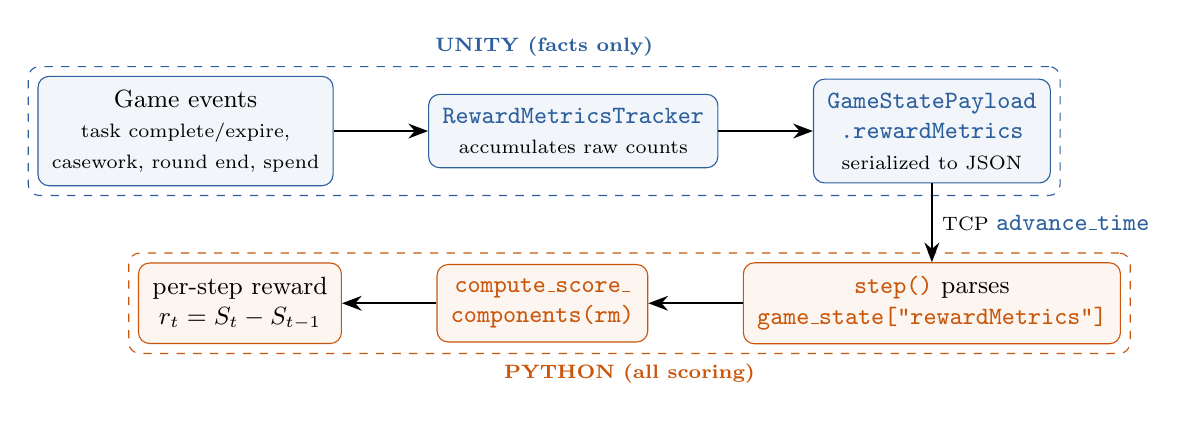
\begin{tikzpicture}[
  node distance=6mm and 12mm,
  box/.style={draw, rounded corners, align=center, inner sep=5pt, font=\small},
  unitybox/.style={box, draw=unityblue, fill=unityblue!6, text=black},
  pybox/.style={box, draw=pyorange, fill=pyorange!6, text=black},
  arr/.style={-{Stealth[length=2.5mm]}, thick}
]
\node[unitybox] (events) {Game events\\{\scriptsize task complete/expire,}\\{\scriptsize casework, round end, spend}};
\node[unitybox, right=of events] (tracker) {\unity{RewardMetricsTracker}\\{\scriptsize accumulates raw counts}};
\node[unitybox, right=of tracker] (payload) {\unity{GameStatePayload}\\\unity{.rewardMetrics}\\{\scriptsize serialized to JSON}};
\node[pybox, below=10mm of payload] (parse) {\py{step()} parses\\\py{game\_state["rewardMetrics"]}};
\node[pybox, left=of parse] (score) {\py{compute\_score\_}\\\py{components(rm)}};
\node[pybox, left=of score] (reward) {per-step reward\\$r_t = S_t - S_{t-1}$};
\draw[arr] (events) -- (tracker);
\draw[arr] (tracker) -- (payload);
\draw[arr] (payload) -- node[right, font=\scriptsize] {TCP \unity{advance\_time}} (parse);
\draw[arr] (parse) -- (score);
\draw[arr] (score) -- (reward);
\begin{scope}[on background layer]
  \node[draw=unityblue, dashed, rounded corners, fit=(events)(tracker)(payload), label={[unityblue,font=\scriptsize\bfseries]above:UNITY (facts only)}] {};
  \node[draw=pyorange, dashed, rounded corners, fit=(reward)(score)(parse), label={[pyorange,font=\scriptsize\bfseries]below:PYTHON (all scoring)}] {};
\end{scope}
\end{tikzpicture}
\caption{Reward pipeline. Unity accumulates raw cumulative quantities and ships them in
\unity{rewardMetrics}; Python computes the composite score and the per-step reward as its
round-over-round delta.}
\label{fig:pipeline}
\end{figure}

% =====================================================================
\section{The Raw Metrics Payload}
% =====================================================================

Every field in \unity{rewardMetrics} is a \emph{cumulative-to-date} quantity, assembled by
\unity{BuildPayload()} on the \unity{RewardMetricsTracker} and attached to the outgoing state in
\unity{TaskSystem.GetCurrentGameState} (which sets \code{state.rewardMetrics} to the payload).
Table~\ref{tab:metrics} lists each field, the Unity source that updates it, and the triggering
game event.

\renewcommand{\arraystretch}{1.3}
\begin{table}[h]
\centering
\scriptsize
\setlength{\tabcolsep}{5pt}
% break-anywhere code macros, scoped (via the group) to ONLY the tabular so the long
% identifiers never overflow a cell; the caption keeps the normal (non-fragile) macros.
\begingroup
\renewcommand{\unity}[1]{{\color{unityblue}\texttt{\scriptsize\seqsplit{#1}}}}
\renewcommand{\code}[1]{{\texttt{\scriptsize\seqsplit{#1}}}}
\begin{tabular}{>{\raggedright\arraybackslash}p{3.3cm} >{\raggedright\arraybackslash}p{5.1cm} >{\raggedright\arraybackslash}p{6.1cm}}
\toprule
\textbf{Field} & \textbf{Unity source (call site)} & \textbf{Updated when / semantics} \\
\midrule
\unity{foodResolved},\newline\unity{foodFulfilled} &
\unity{RecordTaskResolution}\newline(\code{TaskSystem.cs} 1100 / 1199 / 1276); \unity{AddLateDelivery} (614) &
A Food-tagged Demand/Emergency task resolves. \emph{People-based}: \code{resolved}\,+\!=\,\code{demandQuantity}; \code{fulfilled}\,+\!=\,\code{min(delivered, demand)}. Late deliveries credit fulfillment retroactively (capped at resolved). \\
\unity{lodgingResolved},\newline\unity{lodgingFulfilled} &
\unity{RecordTaskResolution} /\newline\unity{AddLateDelivery} (same paths) &
As above for Lodging-tagged tasks (relocation / housing). \\
\unity{caseworkRequested} &
\unity{RecordCaseworkRequested}\newline(\code{ClientStayTracker.cs} 320) &
A ``Casework Request'' is generated for a client group housed too long; adds \code{group.clientCount} people. \\
\unity{caseworkProcessed} &
\unity{RecordCaseworkProcessed}\newline(\code{ClientStayTracker.cs} 205) &
Clients are removed (sent home) via a staffed casework site; adds the number removed. \\
\unity{cumWorkingWorkers},\newline\unity{cumTrainingWorkers},\newline\unity{cumIdleWorkers} &
\unity{OnRoundEnded}\newline(\code{GlobalClock.cs} 458) snapshots \unity{GetWorkerStatistics} &
At each round end, the working / in-training / free worker counts are summed in, giving cumulative \emph{person-rounds}. \\
\unity{roundsCompleted} & \unity{OnRoundEnded} & Count of simulated rounds elapsed. \\
\unity{daysCompleted} & \unity{GlobalClock}\newline\unity{.GetCurrentDay()} & Current in-game day (worker-capacity denominator). \\
\unity{totalWorkers} & \unity{GetWorkerStatistics}\newline(present workers) & Snapshot of all workers present (working + training + free). \\
\unity{foodSpend},\newline\unity{lodgingSpend},\newline\unity{workerSpend},\newline\unity{caseworkSpend} &
\unity{SatisfactionAndBudget}\newline\unity{.Cumulative*Spend} (tallied in \unity{RemoveBudget} by \unity{SpendCategory}) &
Dollars spent per category. \unity{lodgingSpend} absorbs the recurring motel charge: \unity{MotelCostManager} bills \code{residents} $\times$ \$200/day via \code{RemoveBudget(}\,$\ldots$,\,\code{Lodging)}. \\
\bottomrule
\end{tabular}
\endgroup
\caption{The \unity{rewardMetrics} payload: every field, its originating Unity system, and the
game event that updates it. All quantities are cumulative over the episode.}
\label{tab:metrics}
\end{table}

\paragraph{Two design choices worth highlighting.}
\begin{itemize}[leftmargin=1.4em, itemsep=2pt]
\item \textbf{People-based fulfillment.} Food/Lodging success is measured in \emph{people}, not
tasks: a task that ``completes'' but delivers nobody (e.g.\ an immediate evacuation with no
valid destination) adds to \unity{*Resolved} but not \unity{*Fulfilled}. This makes the
satisfaction ratio track actual service delivered.
\item \textbf{Worker allocation as person-rounds.} Worker use is sampled once per round and
summed, so \unity{cumWorkingWorkers} etc.\ measure occupancy integrated over time, which the
scorer normalizes by the available worker-capacity $\unity{daysCompleted}\times\unity{totalWorkers}$.
\end{itemize}

% =====================================================================
\section{Score Components (Python)}
% =====================================================================

All formulas below are implemented in \py{compute\_score\_components} (\py{arc\_game\_gym\_env\_tcp.py}).
Let $\mathrm{rm}$ denote the \unity{rewardMetrics} dict. Two helpers are used throughout:
\begin{equation}
\clip(x) = \min\!\big(1,\max(0,x)\big),
\qquad
\operatorname{ratio}(n,d) = \begin{cases} n/d & d \neq 0\\[2pt] 0 & d = 0.\end{cases}
\end{equation}

\subsection{Satisfaction (higher is better)}
Each satisfaction term is a clamped needs-met ratio scaled by a unit weight ($w_{\text{food}}=w_{\text{lodging}}=w_{\text{workeruse}}=w_{\text{casework}}=1$):
\begin{align}
\text{sat\_food} &= \clip\!\Big(\operatorname{ratio}(\unity{foodFulfilled},\,\unity{foodResolved})\Big)\, w_{\text{food}}, \\[2pt]
\text{sat\_lodging} &= \clip\!\Big(\operatorname{ratio}(\unity{lodgingFulfilled},\,\unity{lodgingResolved})\Big)\, w_{\text{lodging}}, \\[2pt]
\text{casework\_sat} &= \clip\!\Big(\operatorname{ratio}(\unity{caseworkProcessed},\,\unity{caseworkRequested})\Big)\, w_{\text{casework}}.
\end{align}
The worker-use term blends the three allocation states (utilization counts fully, training half,
idle zero) and normalizes by total worker-capacity:
\begin{align}
\text{capacity} &= \max(\unity{daysCompleted},1)\,\cdot\,\max(\unity{totalWorkers},1), \\[2pt]
\text{sat\_worker\_use} &= \clip\!\left(\frac{w_{\text{work}}\,\unity{cumWorking} + w_{\text{train}}\,\unity{cumTraining} + w_{\text{idle}}\,\unity{cumIdle}}{\text{capacity}}\right) w_{\text{workeruse}},
\end{align}
with $(w_{\text{work}},w_{\text{train}},w_{\text{idle}}) = (1,\,0.5,\,0)$. The total satisfaction is the sum:
\begin{equation}
\boxed{\;\text{satisfaction} = \text{sat\_food} + \text{sat\_lodging} + \text{sat\_worker\_use} + \text{casework\_sat}\;}
\end{equation}

\subsection{Cost-Efficiency (lower is better; subtracted)}
Each cost term is dollars-spent per unit-of-service, scaled by a small weight and \emph{capped}
(not clamped) at $\tau = 1$. Spending with zero service is maximally inefficient and hits the cap:
\begin{equation}
\operatorname{cost}(\text{spend},\,\text{service},\,w) = \min\!\left(\frac{\text{spend}}{\max(\text{service},1)}\,w,\ \tau\right), \qquad \tau = 1.
\end{equation}
\begin{align}
\text{cost\_food} &= \operatorname{cost}(\unity{foodSpend},\ \unity{foodFulfilled},\ w_{c}), \\
\text{cost\_lodging} &= \operatorname{cost}(\unity{lodgingSpend},\ \unity{lodgingFulfilled},\ w_{c}), \\
\text{cost\_worker} &= \operatorname{cost}(\unity{workerSpend},\ \unity{cumWorking},\ w_{c}), \\
\text{cost\_casework} &= \operatorname{cost}(\unity{caseworkSpend},\ \unity{caseworkProcessed},\ w_{c}),
\end{align}
with $w_c = 0.0002$ for all four categories (so \$5000/service saturates the cap). The aggregate is
\begin{equation}
\text{cost\_efficiency} = \text{cost\_food} + \text{cost\_lodging} + \text{cost\_worker} + \text{cost\_casework}.
\end{equation}

\subsection{Composite Score and Per-Step Reward}
\begin{equation}
\boxed{\;S = \text{satisfaction} - \text{cost\_efficiency}\;}
\end{equation}
$S$ is a cumulative-to-date quantity. The Gym reward at round $t$ is its round-over-round delta,
which telescopes so the undiscounted return equals the final score:
\begin{equation}
r_t = S_t - S_{t-1}, \qquad \sum_{t=1}^{T} r_t = S_T - S_0.
\end{equation}

\begin{table}[h]
\centering
\footnotesize
\renewcommand{\arraystretch}{1.15}
\begin{tabular}{llll}
\toprule
\textbf{Weight} & \textbf{Value} & \textbf{Weight} & \textbf{Value} \\
\midrule
$w_{\text{food}},w_{\text{lodging}},w_{\text{workeruse}},w_{\text{casework}}$ & $1.0$ & $w_c$ (all cost categories) & $0.0002$ \\
$w_{\text{work}}$ (working) & $1.0$ & cost cap $\tau$ & $1.0$ \\
$w_{\text{train}}$ (in-training) & $0.5$ & $w_{\text{idle}}$ (idle) & $0.0$ \\
\bottomrule
\end{tabular}
\caption{Reward weights (\py{REWARD\_WEIGHTS}). All scoring constants live in Python and are
retunable without rebuilding Unity.}
\label{tab:weights}
\end{table}

\paragraph{Reading the score.} Satisfaction has a natural ceiling of $4.0$ (four unit-weighted
terms each $\le 1$); cost-efficiency can subtract up to $4.0$ (four capped terms). In practice
strong policies land near $S \approx 2$--$2.5$: high needs-met ratios minus modest per-service cost.
Termination occurs if in-game satisfaction drops to $0$; episodes otherwise truncate at the
round limit.

\end{document}
